
\subsection{Allocator Versions}

To facilitate the support for multiple versions of the allocator with a configurable design, the primary TLSF implementation has been abstracted into a base class named \texttt{TLSFBase}. The base class implements all parts described in the TLSF design except for the \texttt{free()} method, which varies greatly between use-cases and should therefore be implemented optimally for every new configuration. For each configuration, the base class enables the user to specify the allocator's behavior through a set of configuration variables, which includes:

\begin{enumerate}
  \item Number of first- and second-level indexes.
  \item Whether to use second-level or not.
  \item Minimum block size.
  \item Whether to use deferred coalescing.
  \item Block header length.
\end{enumerate}

\subsection{New Bitmap Design}

Summarizing the insight from Section~\ref{sec:adaptations:reduced_allocation_range} regarding the number of required first- and second-levels, desire to use a single 64-bit bitmap and large-list, we can construct a new bitmap representation, as shown in Figure~\ref{fig:bitmap_flattening}. The new bitmap disregards the literal notion of ``Two Level'' from Two Level Segregated Fit and flattens the first- and second-level bitmaps to a single bitmap. The new bitmap is indexed using the formula: 
\[
    \text{bitmap\_index($f, s$)} = f \cdot 4 + s
\]
where $f$ and $s$ are the first- and second-level indexes respectively. Additionally, the lowest size classes have been placed at the least significant bits of the bitmap to make searching for the next non-empty free-list efficient using the find-first-set bit instruction.

\begin{figure}[H]
    \centering
    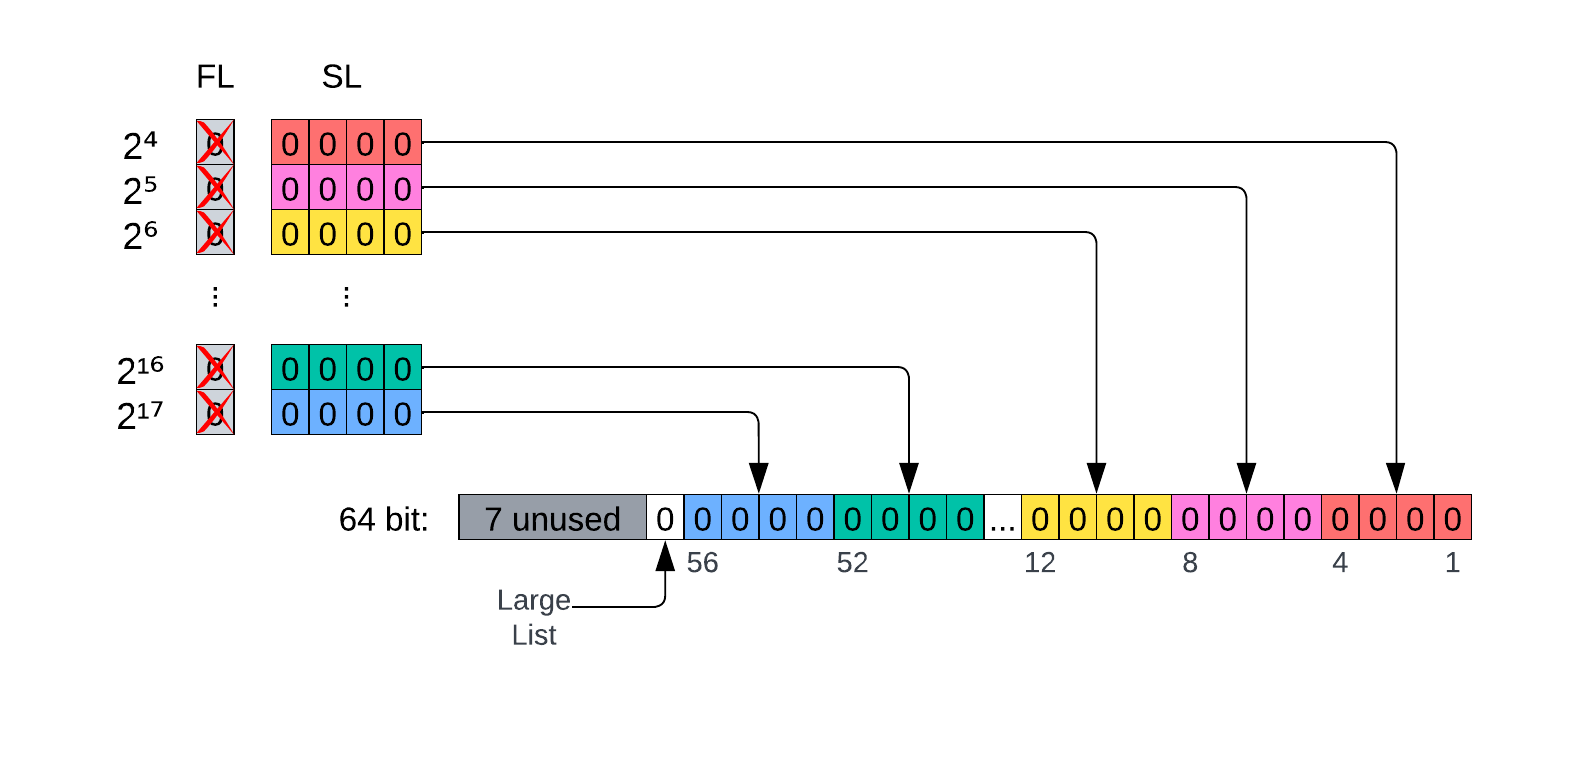
\includegraphics[width=1\textwidth]{figures/bitmap_flattening.png}
    \caption{Flattening of the 2D-matrix representation of TLSF bitmaps into a single 64-bit value. The first-level bitmap is disregarded in favor of indexing the new flattened bitmap using the first-level value instead. The number of first-levels are 14, indicated by bits of the same color belonging to the same first-level. The number of second-levels are 4, as indicated by the same number of colored bits.}
    \label{fig:bitmap_flattening}
\end{figure}

The correlation between the bitmap and the free-lists is depicted in Figure~\ref{fig:bitmap_relationship}, adhering closely to the original TLSF design. However, the adaptation now more efficiently determines the relevant free-list by looking in the single bitmap, not two bitmaps as in the original design.

\begin{figure}[H]
    \centering
    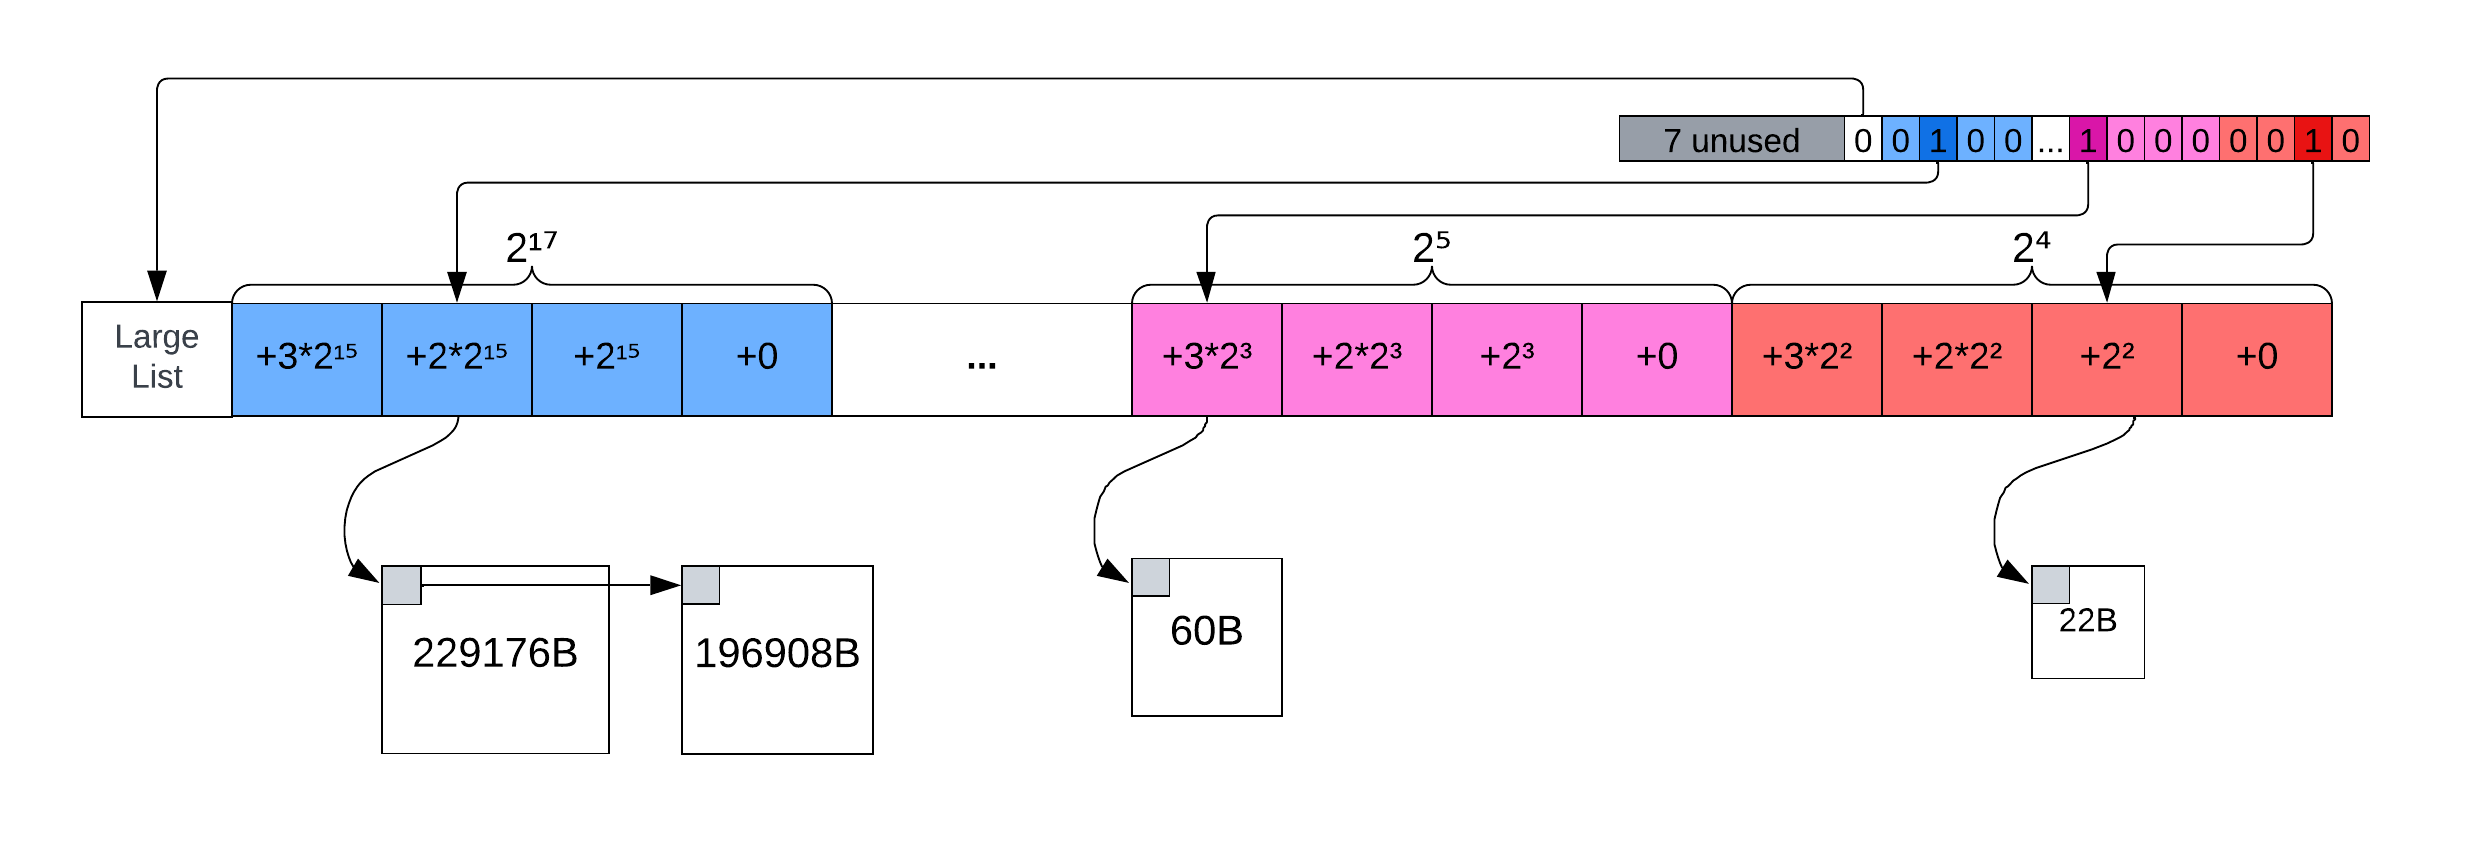
\includegraphics[width=1\textwidth]{figures/bitmap_relationship.png}
    \caption{Relationship between the new bitmap representation and accessing the corresponding free-lists.}
    \label{fig:bitmap_relationship}
\end{figure}

\subsection{Block Header Adjustments and 0-byte Header}
\label{sec:adaptations_impl:0-byte-header}

The block header, as designed in the reference implementation, is shown in Figure~\ref{fig:blockheader_adap_reference}. Here, the size and previous physical pointer (prev\_phys) are constant and the next and prev pointers are only used in the unused part of free blocks, and unused for allocated blocks. In contrast, Figure~\ref{fig:blockheader_adap_general} shows the adapted block header for the general version of the allocator. In this version, all four fields are used for both free and allocated blocks since the previous physical pointer has been rearranged to the end of the header. Rearranging the previous physical pointer this way allows us to have the block header for optimized blocks, as shown in Figure~\ref{fig:blockheader_adap_optimized}, while using the same block header definition as the general version. 

As stated in Section~\ref{sec:adaptations:block-header-adjustments}, the size field can be ignored for allocated blocks if the user of the allocator keeps track of its size somewhere else and provides that information upon freeing a block. Additionally, to further minimize footprint, the next and prev pointers have been converted to offsets in the optimized version, allowing them to be 32 bits each. Both the size field and next/prev pointers being unused for allocated blocks and stored in the unused parts for free blocks. In the optimized version, this results in the header taking up 0 bytes for allocated blocks and 16 bytes for free blocks.

\begin{figure}[H]
    \centering
    \begin{subfigure}[b]{0.3\textwidth}
        \centering
        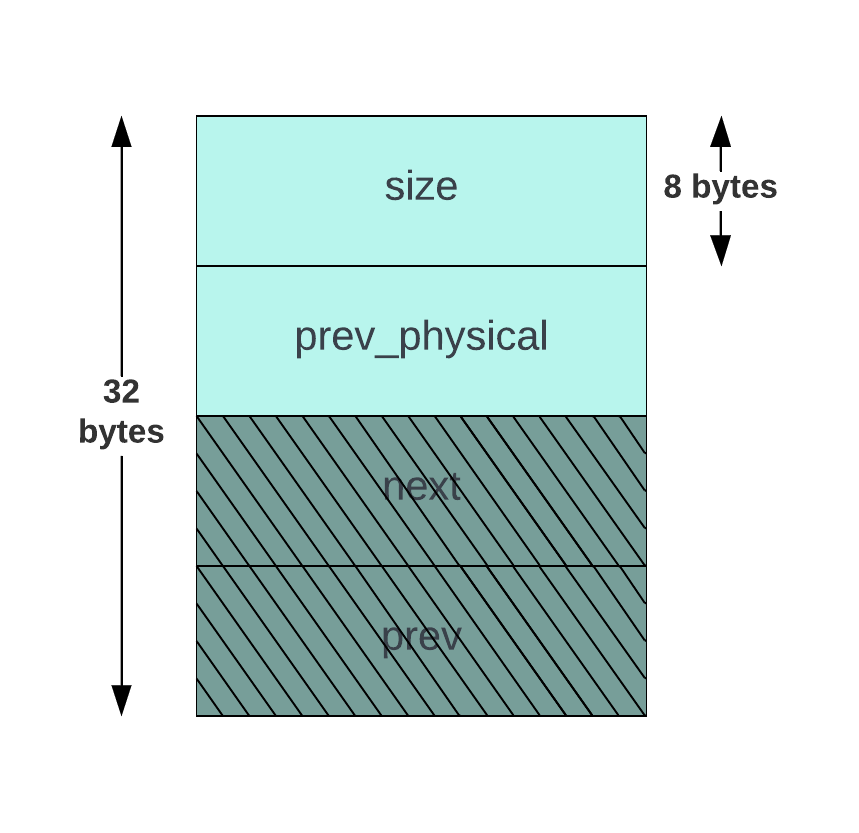
\includegraphics[width=\textwidth]{figures/blockheader_adap_reference.png}
        \caption{Reference implementation block header.}
        \label{fig:blockheader_adap_reference}
    \end{subfigure}%
    \hfill
    \begin{subfigure}[b]{0.3\textwidth}
        \centering
        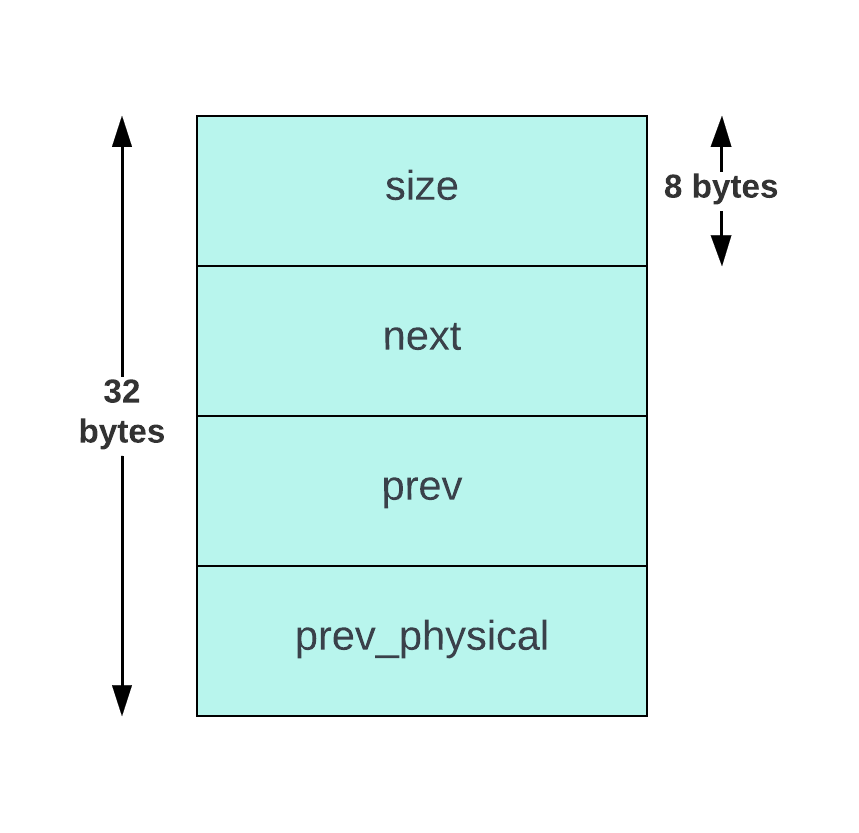
\includegraphics[width=\textwidth]{figures/blockheader_adap_general.png}
        \caption{Adapted general block header.}
        \label{fig:blockheader_adap_general}
    \end{subfigure}%
    \hfill
    \begin{subfigure}[b]{0.3\textwidth}
        \centering
        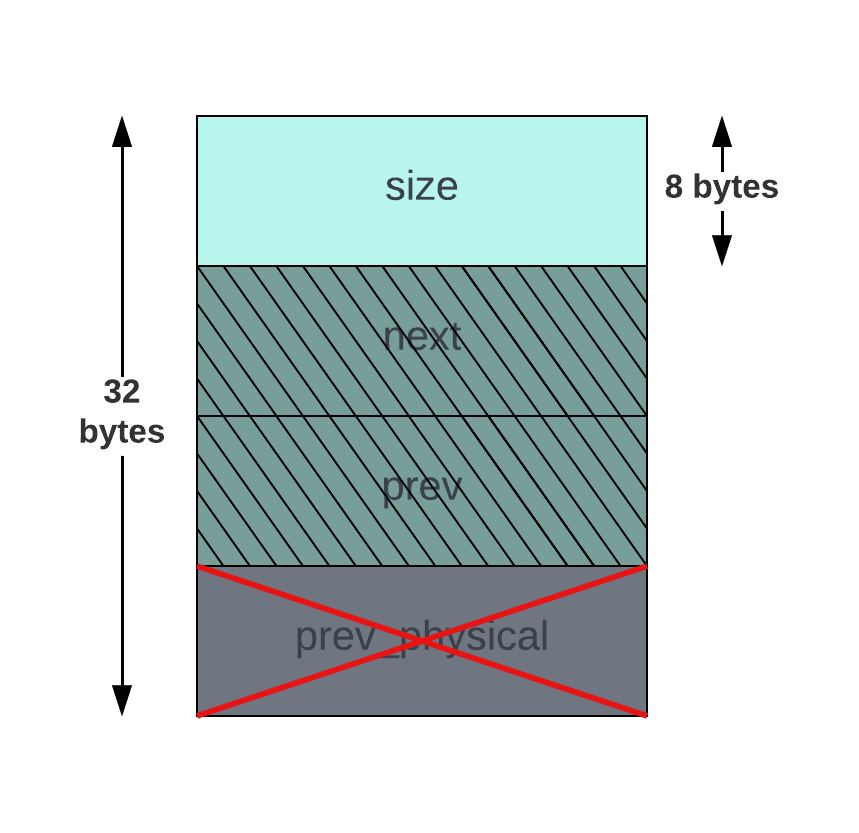
\includegraphics[width=\textwidth]{figures/blockheader_adap_optimized.png}
        \caption{Adapted optimized block header.}
        \label{fig:blockheader_adap_optimized}
    \end{subfigure}
    \caption{Overview of block header contents and adaptations. Dashed fields are only unused in the unused part of free blocks and crossed out fields are unused.}
    \label{fig:blockheader_adaptations}
\end{figure}

\subsection{Concurrency Implementation}
\label{sec:adaptations_impl:concurrency}

For the optimized version we have implemented concurrency in a lock-free manner. To do this, we have made a few simplifications to reduce the complexity of the inner data structures that are used in the allocator. The major change is that the pointer to the previous free block inside block headers is ignored completely, which changes the appearance of the free-lists to a singly-linked list from a doubly-linked list. Furthermore, the singly-linked list will only be allowed to be altered from the head, essentially making it a stack. This is a reasonable approach since elements are only potentially removed from an arbitrary position inside the free-list if we allow for immediate coalescing, which is not the case in the optimized version.

M. Herlihy and N. Shavit~\cite[Chapter 11]{artofmpprogramming} describes the design and inner-workings of a lock-free stack from which the concurrent implementation of the allocator is largely based on. For reference, we will go over how a lock-free stack work and how it connects to the data structure inside the allocator.

A stack only requires two operations: \texttt{push()} and \texttt{pop()}, which are named \texttt{insert()} and \texttt{remove()} in the allocator to stay consistent with their meaning from the general version. The insert operation replaces the head of the stack, or free-list, with a new block, whilst the remove operation removes the head of the free-list and replaces it with the next block, if any, in the free-list. In order to make the allocator work in a thread-safe manner, we only need to make these two operations concurrent, since all other operations in the allocator can be done independently of other threads.

To be able to operate on the free-list concurrently without locks, we will use the atomic operations \texttt{load()}\footnote{\url{https://en.cppreference.com/w/cpp/atomic/atomic/load}} and \texttt{compare\_exchange()}\footnote{\url{https://en.cppreference.com/w/cpp/atomic/atomic/compare_exchange}}, provided in the C++ standard library. \texttt{load()} returns the current value of an atomic variable and \texttt{compare\_exchange()} compares the value of a variable with an expected value, and if they are equal, it is replaced by another value.

\subsubsection{Solving The ABA Problem}
\label{sec:adaptations_impl:aba_problem}

% To remind, the ABA problem happens when a thread reads the value it wants to change with compare-and-swap, gets preempted, and when it resumes the actual value of the pointer happens to be equal to what the thread read before. Therefore the compare-and-swap operation may succeed despite data structure modifications possibly done by other threads during the preemption time.

A strategy for solving the ABA problems is ensuring that all values, or pointers in the allocator, are inherently unique and used only once. This approach enables the detection of changes during thread preemption. However, inside the allocators, pointers to blocks are not unique and can be inserted and removed any number of times. A way around this is to apply a so-called version tag to each pointer, which allow us to uniquely identify pointers by their version.

Version tagging is described by D. Dechev et al.~\cite{bjarne_aba} as a common and effective solution for the ABA problem. However, it is stated that due to how compare-and-swap (CAS) (\texttt{compare\_exchange()} in C++) work, it is desirable to store the pointer and version tag in a single word, i.e 8-bytes on a 64-bit system. When using the allocator for pages in ZGC, this is not a problem as we can apply the same principle as in Section~\ref{sec:adaptations_impl:0-byte-header} to convert 64-bit pointers to 32-bit offsets. Making this conversion allows us to store the version tag in the remaining 32-bits of the word, as illustrated in Figure~\ref{fig:concurrent_head_bits}.

\begin{figure}[H]
    \centering
    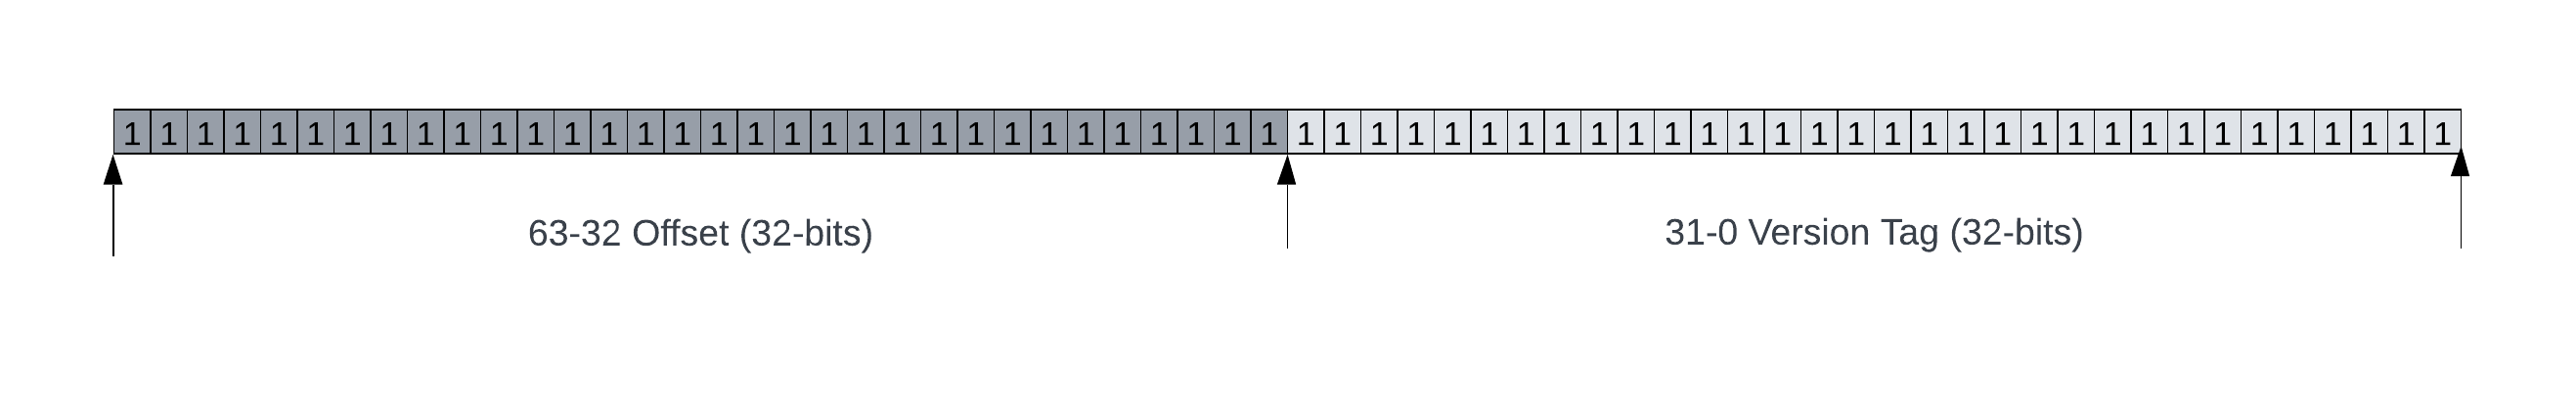
\includegraphics[width=1\textwidth]{figures/concurrent_head_bits.png}
    \caption{Bit representation of a free-list head in the allocator. The 32 most significant bits are used to store the offset and the 32 least significant bits are used to store the version tag.}
    \label{fig:concurrent_head_bits}
\end{figure}

\subsubsection{Inserting a block}

The process of concurrently inserting a block into a free-list is outlined in Algorithm~\ref{algorithm:concurrent_insert_block}. Notably, both the \texttt{load()} and \texttt{compare\_exchange()} operations are atomic. It is essential to recognize that, between loading the old head from the free-list and executing the \texttt{compare\_exchange()} operation, the new head must be assembled using data from the old head. However, there exists a potential issue wherein the thread responsible for this construction may be preempted, allowing another thread to modify the head during this time. To address this, if the \texttt{compare\_exchange()} operation fails, the thread will loop and create a new head until it successfully performs the operation.

\begin{algorithm}[H]
    \SetAlgoLined
    \SetKwInOut{Input}{}
    \SetKwRepeat{Do}{do}{while}

    \SetKwFunction{FMain}{insert\_block}
    \SetKwProg{Fn}{Function}{:}{\KwRet}
    \Fn{\FMain{blk}}{
    mapping = get\_mapping(blk->size)\;
    \Do{blocks[mapping].compare\_exchange(old\_head, new\_head)}{ 
        old\_head = blocks[mapping].load()\;

        version, old\_head\_ptr = split\_tagged\_head(old\_head)\;
        blk->next = old\_head\_ptr\;

        new\_head = construct\_new\_head(inserted\_block, version + 1)
    }
    update\_bitmap(mapping)\;
    }
\label{algorithm:concurrent_insert_block}
\caption{Concurrent insertion of a block into the head of a free-list.}
\end{algorithm}

\subsubsection{Removing a block}

The process of concurrently removing a block from a free-list, as illustrated in Algorithm~\ref{algorithm:concurrent_remove_block}, is similarly defined to block insertion. The main difference is that instead of a while-loop, removal involves replacing the head with the next block in the list, possibly a NULL value.

If the \texttt{compare\_exchange()} operation fails when removing a block, there is no guarantee that the same free-list contain additional blocks. In cases where thread preemption occurs during removal, other threads might exhaust the free-list, which will make further operations fail. To solve this, \texttt{remove\_block()} either succeeds or fails, without looping until successful like \texttt{insert\_block()} does. Consequently, the caller must recalculate the mapping and call \texttt{remove\_block()} again.

\begin{algorithm}[H]
    \SetAlgoLined
    \SetKwInOut{Input}{}

    \SetKwFunction{FMain}{remove\_block}
    \SetKwProg{Fn}{Function}{:}{\KwRet}
    \Fn{\FMain{mapping}}{
        old\_head = blocks[mapping].load()\;
        version, old\_head\_ptr = split\_tagged\_head(old\_head)\;
        new\_head\_ptr = get\_next\_block(old\_head\_ptr)\;
        new\_head = construct\_new\_head(new\_head\_ptr, version + 1)\;

        \uIf{blocks[mapping].compare\_exchange(old\_head, new\_head)} {
            update\_bitmap(mapping)\;
            \KwRet new\_head\_ptr
        } \Else {
            \KwRet nullptr
        }

    }

\label{algorithm:concurrent_remove_block}
\caption{Concurrent removal of the head of a free-list.}
\end{algorithm}

%%% Local Variables:
%%% mode: latex
%%% TeX-master: "main"
%%% End:
